\section{09.10.2024}{To be named}

\begin{lemma}{Milnora-\v{S}varca}{}
  Niech $X$ będzie właściwą przestrzenią geodezyjną a $\Gamma$ grupą działającą na $X$ przez izometrie właściwie i kozwarcie. Wówczas $\Gamma$ jest skończenie generowalna i quasi-izometryczna z $X$. Dokładniej, $\forall\;x_0\in X$ odwzorowanie $\Gamma\to X$ określone przez $\gamma\mapsto \gamma\cdot x_0$ jest quasi-izometrią.
\end{lemma}

\begin{proof}
  Wybierzmy $x_0\in X$. Z kozwartości tego działania, istnieje promień $R>0$ taki, że dla kuli $B=B_R(x_0)$ o środku w $x_0$ taki, że rodzina przesunięć kuli $\{g\cdot B\;:\; g\in\Gamma\}$ jest pokryciem $X$. Rozważmy zbiór $S=\{s\in\Gamma\;:\;s\neq1,s\cdot B\cap B\neq \emptyset\}$ niewielkich przesunięć kuli $B$. Z właściwości działania oraz z właściwości przestrzeni $X$, zbiór $S$ jest skończony. Ponadto, zbiór jest ten jest symetryczny $S=S^{-1}$ ($s\in S\implies s^{-1}\in S$), bo jeśli $s\cdot B\cap S\neq \emptyset$ to również $s^{-1}\cdot (s\cdot B\cap B)\neq \emptyset$.

  Określamy $v:=\inf\{d(B, g\cdot B)\;:\;g\in \Gamma-S-\{1\}\}$ czyli najmniejsza odległość kuli od jej rozłącznych z nią przesunięć.

  \textbf{Clam 1:} $v>0$

  Dla każdego $g\in\Gamma-S-\{1\}$ wiemy, że $d(B, g\cdot B)>0$. Gdyby to infimum $v=0$, to mielibyśmy ciąg parami różnych elementów $g_n\in\Gamma$ takich, że $d(B, g_n\cdot B)\searrow 0$ maleją do $0$. Stąd mielibyśmy punkty $z_n\in B$ takie, że $d(z_n, g_n\cdot B)\searrow 0$ (jako punkty prawie realizujące odległość między zbiorami). Istnieje podciąg $n_k$ taki, że $z_{n_k}\in z_0\in B$, a stąd $d(z_0, g_n\cdot B)\searrow 0$. To oznacza, że $B_{2R}(x_0)$ przecina niepusto nieskończenie wiele spośród przesunięc $g_n\cdot B_{2R}(x_0)$, a to jest sprzeczne z właściwością działania.

  \textbf{Clam 2:} $S$ generuje $\Gamma$ oraz dla każdego $\gamma\in\Gamma$
  $$\frac{1}{\lambda}d_X(x_0, \gamma\cdot x_0)\leq d_S(1, \gamma)\leq\frac{1}{r}d_X(x_0,\gamma\cdot x_0)+1,$$
  gdzie $\lambda:=\max_{s\in S}d_X(x_0, s\cdot x_0)$.

  I scenariusz:

  \begin{center}
    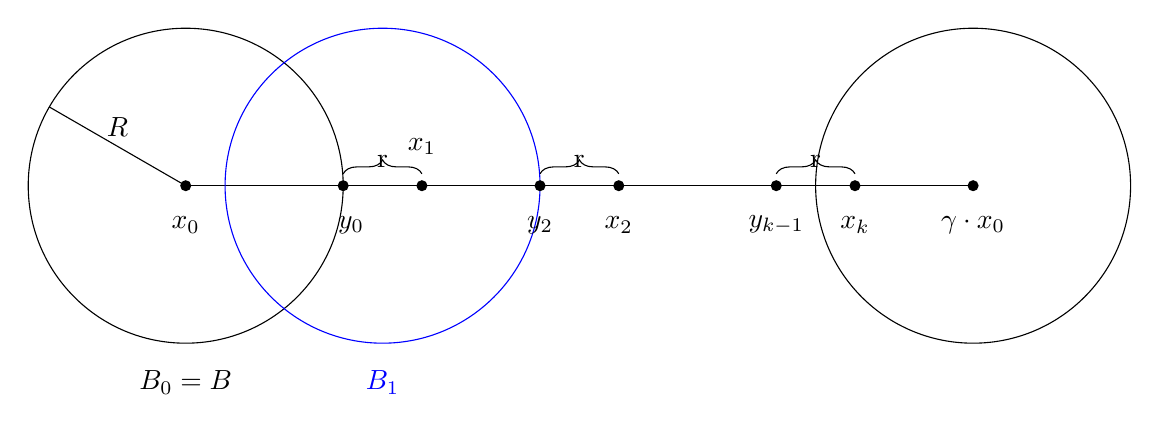
\begin{tikzpicture}
    \fill (0,0) circle (2pt);
    \draw (0,0) circle (2);
  \fill (10, 0) circle (2pt);
  \node at (0, -.5) {$x_0$};
  \node at (10, -.5) {$\gamma\cdot x_0$};
  \draw (0,0)--({2*cos(150)}, {2*sin(150)}) node[midway, above] {$R$};
  \draw(0,0)--(10, 0);
\fill (2, 0) circle (2pt);
\node at (2.1, -.5) {$y_0$};
\fill (3, 0) circle (2pt);
\draw[blue] (2.5, 0) circle (2);
\node at (2.5, -2.5) {$\color{blue}B_1$};
\node at (0, -2.5) {$B_0=B$};
\node at (3, .5) {$x_1$};
\draw [decorate,decoration={brace,amplitude=5pt,raise=1ex}] (2,0) -- (3,0) node[midway,yshift=2ex]{r};

\draw(10,0) circle (2);
\fill (8.5, 0) circle (2pt);
\node at (8.5, -.5) {$x_k$};
\fill (7.5, 0) circle (2pt);
\node at (7.5, -.5) {$y_{k-1}$};
\draw [decorate,decoration={brace,amplitude=5pt,raise=1ex}] (7.5,0) -- (8.5,0) node[midway,yshift=2ex]{r};

\fill(4.5, 0) circle (2pt);
\node at (4.5, -.5) {$y_2$};
\draw [decorate,decoration={brace,amplitude=5pt,raise=1ex}] (4.5,0) -- (5.5,0) node[midway,yshift=2ex]{r};
\fill(5.5, 0) circle (2pt);
\node at (5.5, -.5) {$x_2$};
    \end{tikzpicture} 
  \end{center}
  II scenariusz
  \begin{center}
    \begin{tikzpicture}
    \fill (0,0) circle (2pt);
    % \draw (0,0) circle (2);
  \node at (0, -.5) {$x_0$};
  \draw(0,0)--(10, 0);
\fill(10, 0) circle (2pt);

\draw(7.5,0) circle (2);
\fill (8.5, 0) circle (2pt);
\node at (8.5, -.5) {$x_k$};
\fill (9.5, 0) circle (2pt);
\node at (9.5, -.5) {$y_{k}$};
\draw [decorate,decoration={brace,amplitude=5pt,raise=1ex}] (9.5,0) -- (10.5,0) node[midway,yshift=2ex]{r};
\node at (10.5, -.5) {$\gamma\cdot x_0$};

    \end{tikzpicture}
  \end{center}
  Niech $y_0$ będzie punktem na geodezyjnej $[x_0, \gamma\cdot x_0]=\eta$ z kuli $B$ najdalszy od $x_0$ na tej geodezyjnej. W odległości $r$ od $y_0$ obierzmy punkt $x_1$.
  Wtedy odcinek $(y_0, x_1)\subseteq\eta\subseteq \bigcup_{s\in S}s\cdot B$, ale to jest zbiór domknięty, z czego wynika, że $x_1\in \bigcup_{s\in S} s\cdot B$, czyli $x_1\in s_1\cdot B$. Iterujemy się tak aż kulą $B_k=s_ks_{k-1}...s_1 \cdot B$ trafimy w $\gamma\cdot x_0$.

  % {\large\color{red}DORYSOWAC II scenariusz}

  W scenariuszu I mamy $\gamma\cdot B\cap s_k...s_1 \cdot B\neq\emptyset$, bo $\gamma x_0\in \gamma\cdot B$ oraz $\gamma x_0\in s_k...s_1\cdot B$. W takim razie $s_1^{-1}...s_k^{-1}\gamma\cdot B\cap B\neq\emptyset$. Czyli zachodzi jedna z równości
  \begin{enumerate}
    \item $s1^{-1}...s_k^{-1}\gamma=1\implies \gamma=s_k...s_1$
    \item $s_1^{-1}...s_k^{-1}\gamma=s_{k+1}\in S\implies \gamma=s_k...s_1s_{k+1}$
  \end{enumerate}

  W scenariuszu II $d(\gamma x_0, s_k...s_1\cdot B)<v\implies d(x_0,\gamma^{-1}s_k...s_1\cdot B)<r\implies d(B, \gamma^{-1}s_k...s_1\cdot B)<r$. W takim razie znowu zachodzi jedna z równości
  \begin{enumerate}
    \item $s1^{-1}...s_k^{-1}\gamma=1\implies \gamma=s_k...s_1$
    \item $s_1^{-1}...s_k^{-1}\gamma=s_{k+1}\in S\implies \gamma=s_k...s_1s_{k+1}$
  \end{enumerate}

  Dla uzyskania prawej nierówności, zauważamy, że w obu scenariuszach 
  $d_S(1,\gamma)\leq k+1\leq \frac{1}{r}d_X(x_0,\gamma\cdot x_0)+1$, bo $d(x_0, \gamma\cdot x_0)\geq k\cdot r$ bo tyle razy udało nam się odłożyć $r$ na geodezyjnej.

  Jeśli $d_S(1,\gamma)=m$, a $\gamma=s_1...s_m$, to wówczas
  $$d_X(s_1,...,s_k\cdot x_0,s_1...s_{k-1}\cdot x_0)=d_X(s_k\cdot x_0,x_0)\leq \lambda.$$
  Z nierówności trójkąta 
  $$d(\gamma\cdot x_0,x_0)=d(s_1...s_k\cdot x_0,x_0)\leq m\cdot \lambda=d_S(1,\gamma)\cdot\lambda$$
  co właściwie kończy dowód Claim 2. 

  Pozostaje nam udowodnienie quasi-izometryczności $f(\gamma)\to \gamma\cdot x_0$, które staje się \textbf{Claim 3}.

  Z lewo niezmienniczości metryki słów $d_S$ wiemy, że $d_S(\gamma_1, \gamma_2)=d_s(1, \gamma_1^{-1}\gamma_2)$, czyli wszystkie dystanse wyrażają się jako dystanse od $1$. Z kolei z lewo-$\Gamma$-niezmienniczości metryki $d_X$ na $X$ mamy 
  $$d_X(f(\gamma_1), f(\gamma_2))=d_X(\gamma_1\cdot x_0,\gamma_2\cdot x_0)=d_X(x_0,\gamma_1^{-1}\gamma_2\cdot x_0).$$
  Nierówności z \textbf{Claim 2} otrzymujemy następujący wariant nierówności
  $$\frac{1}{\lambda}d_X(f(\gamma_1), f(\gamma_2))\leq d_S(\gamma_1,\gamma_2)\leq \frac{1}{r}\cdot d_X(f(\gamma_1), f(\gamma_2))+1$$
  Stąd wynika, że 
  $$r d_S(\gamma_1,\gamma_2)-r\leq d_x(f(\gamma_1),g(\gamma_2)\leq \lambda d_S(\gamma_1,\gamma_2)$$
  i $f$ jest quasi-izometrycznym włożeniem dla $C=\max(\lambda, \frac{1}{r})$ i $L=r$.

  Ponadto, obraz $f(\Gamma)$ jest $R$-gęsty (dla $R$ promienia z początku dowodu) w $X$, bo dla każdego $x\in X$ istnieje $\gamma\in\Gamma$ takie, że $x\in\gamma\cdot B_R(x_0)=B_R(\gamma\cdot x_0)$. Czyli $d_X(x, \gamma\cdot x_0)\leq R$, ale $\gamma\cdot x=f(x)$. Stąd $f$ jest quasi-izometrią.
\end{proof}

Niewszystkie quasi-izometryczne grupy są współmierne.

\begin{example}[m]
\item Grupy podstawowe $\pi_1(M_1)$, $\pi_1(M_2)$ zamkniętych $3$-wymiarowych rozmaitości hiperbolicznych $M_1$, $M_2$ o niewspółmiernych (jedna nie jest iloczynem drugiej przez liczbę wymierną) objętościach $vol(M_i)$.

  Wiadomo, że istnieje wiele klas niewspółmierności wśród objętości takich rozmaitości.

  \begin{theorem}{Mostowa o sztywności [1968]}{}
    Dwie zamknięte hiperboliczne rozmaitości o izomorficznych grupach podstawowych są izometryczne. W szczególności, mają jednakowe objętości.
  \end{theorem}

  Załóżmy nie wprost, że $\pi_1(M_1)$ i $\pi_1(M_2)$ są współmierne, to wówczas mielibyśmy wspólną podgrupę skończonego indeksu $H< \pi_1(M_1)$, $H<\pi_1(M_2)$. Niech $\overline{M}_1$ i $\overline{M}_2$ będą nakryciami $M_1,M_2$ wyznaczone przez $H$. Skoro indeks grupy jest skończony, to nakrycia też takie są, a więc $\overline{M}_i$ są zwarte i z podniesionymi metrykami Riemanna, a więc są w dalszym ciągu hiperboliczne.

  Z teorii nakryć wiemy, że $\pi_1(\overline{M}_1)\cong H\cong \pi_1(\overline{M}_2)$. Stąd wynika, że $\overline{M}_1$ jest izometryczna z $\overline{M}_2$, a więc ich objętości są równe sobie. Ale 
  $$vol(\overline{M}_i)=(\underbrace{\text{krotność nakrycia}}_{=[\pi_1(M_i):H]})\cdot vol(M_i)$$
  stąd 
  $$\frac{vol(M_1)}{vol(M_2)}=\frac{[\pi_1(M_1):H]}{[\pi_1(M_2):H]}$$
  daje sprzeczność z niewspółmiernością.
\item Niech $G_A$ będzie produktem półprostym $\Z\ltimes_A\Z^2$, gdzie $A:\Z^2\to \Z^2$ jest zadane macierzą $A\in Sl_2\Z$. Chcemy, żeby $A$ było macierzą hiperboliczną (tzn. $|tr(A)|>2$) posiadającą dwie różne rzeczywiste wartości własne, odwrotne do siebie. Wówczas grupa $G_A$ jest kratą (podgrupą dyskretną i kozwartą) w pewnej grupie Liego $Sol=(\R^3,\cdot)$, gdzie mnożenie jest zadane jako
  $$(x,y,z)\cdot(a,b,c)=(e^z\cdot a,e^{-z}\cdot b,c+z)$$
\end{example}

